% !TeX spellcheck = en_US
\documentclass[letterpaper,12pt,twoside]{report}
\usepackage{fancyhdr}
\usepackage{fullpage}
\usepackage{tikz}
\usepackage{amsmath}

\begin{document}
	\pagestyle{fancy}
	\fancyhf{}
	\fancyhead[L]{Day 17}
	\fancyhead[R]{\textit{The Calendar Project}}
	\fancyfoot[L]{Citations Involved: none}
	
	% Problem
	\paragraph{Problem}
	\begin{quote}
		\textsf{Rectangle $ABCD$ lies in the y,z-plane with $A(0,10,0)$, $B(0,10,25)$, and $D(0,k,0)$; $k>10$. The
			rectangle is rotated
			about the z-axis to create
			a hollow cylinder. The
			rectangle is also rotated
			about the y-axis to create
			a solid cylinder. If the
			volumes of the two solids are equal, what
			is the value of $k$?}
	\end{quote}
	
	% Graphics
	
		\begin{minipage}{0.6\linewidth}
			\begin{center}
		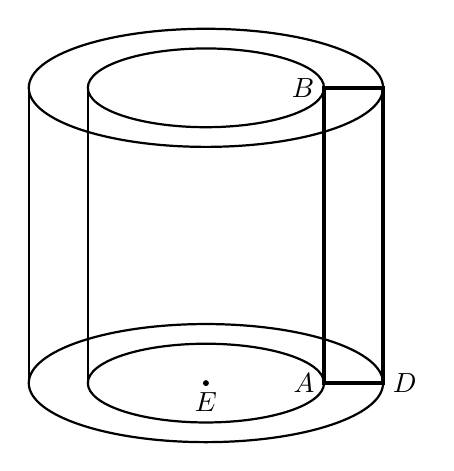
\begin{tikzpicture}[scale=0.15]
		\draw[thick] (-10,25) circle [x radius=15, y radius=5];
		\draw[thick] (-10,25) circle [x radius=10, y radius=3.333333];
		\draw[thick] (-10,0) circle [x radius=15,y radius=5];
		\draw[thick] (-10,0) circle [x radius=10, y radius=3.333333];
		
		\draw[thick] (-20,25) -- (-20,0);
		\draw[thick] (0,25) -- (0,0);
		\draw[thick] (-25,25) -- (-25,0);
		\draw[thick] (5,25) -- (5,0);
		\draw[ultra thick] (0,25) -- (5,25) -- (5,0) -- (0,0) -- cycle;
		\node[left] at (0,0) {$A$};
		\node[left] at (0,25) {$B$};
		\node[right] at (5,0) {$D$};
		\draw[fill] (-10,0) circle [radius=0.2];
		\node[below] at (-10,0) {$E$};
		
		\end{tikzpicture}
		\end{center}
	\end{minipage}
\begin{minipage}{0.3\linewidth}
	\begin{center}
		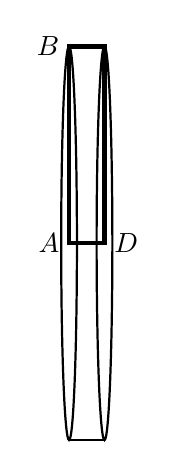
\begin{tikzpicture}[scale=0.1]
		\draw[ultra thick] (10,25) -- (14.5,25) -- (14.5,0) -- (10,0) -- cycle;
		\node[left] at (10,0) {$A$};
		\node[left] at (10,25) {$B$};
		\node[right] at (14.5,0) {$D$};
		
		\draw[thick] (14.5,0) circle [x radius=1, y radius=25];
		\draw[thick] (10,0) circle [x radius=1, y radius=25];
		\draw[thick] (14.5,-25) -- (10,-25);
		
		\end{tikzpicture}
		\end{center}
		\end{minipage}
	
	% Reasoning
	\paragraph{Reasoning}
	\begin{quotation}
		
		The width ($AD$) and height ($AB$) of rectangle $ABCD$ are determined using the Distance Formula: $AD=\sqrt{(0-0)^2+(k-10)^2+(0-0)^2}=\sqrt{(k-10)^2}=k-10$, $AB=\sqrt{(0-0)^2+(10-10)^2+(25-0)^2}=\sqrt{25^2}=25$.
		
		The base of the hollow cylinder is a ring. Its area can be determined by subtracting the area of the inner circle from the area of the outer circle. Since the rectangle is rotated about the z-axis to produce the hollow cylinder, the center of the circles that form the base is the point where the z-axis intersects the plane containing the base; the center has coordinates $(0,0,0)$. Name this point $E$. The radii of the two concentric circles are determined using the Distance Formula: $EA=\sqrt{(0-0)^2+(10-0)^2+(0-0)^2}=\sqrt{10^2}=10$ and  $ED=\sqrt{(0-0)^2+(k-0)^2+(0-0)^2}=\sqrt{k^2}=k$ where $EA$ represents the radius of the inner circle and $ED$ represents the radius of the outer circle. The area formula for a circle is $r^2\pi$ where $r$ is its radius (1); this is applied to determine the areas of the two circles: $10^2\pi=100\pi$ for the inner circle, $k^2\pi$ for the outer circle. The area of the ring (the hollow cylinder's base) is therefore $k^2\pi-100\pi=(k^2-100)\pi$.
		
		The height of the hollow cylinder is represented by $AB$, which is previously determined to be 25. The volume formula for a cylinder is $Bh$ where $B$ is the area of its base (2); this is applied to determine the volume of the hollow cylinder: $Bh=25(k^2-100)\pi$.
		
		In the solid cylinder, $A$ and $D$ are on the y-axis. Since this cylinder is created by rotating the rectangle about the y-axis, the center of its bases are $A$ and $D$. Their radius can thus be represented by $AB$, or the rectangle's height. Using the area formula for a circle ($r^2\pi$) (1), the area of the solid cylinder's base is determined to be $25^2\pi=625\pi$. The height of the solid cylinder is represented by width of the rectangle, which is $AD=k-10$. The volume formula for a cylinder is $Bh$ where $B$ is the area of its base (2); its application to the solid cylinder yields $Bh=625\pi(k-10)$.
		
		Given that the volumes of the cylinders are equal, $25(k^2-100)\pi=625\pi(k-10)$. This is solved for $k$ as follows:
		
		\begin{center}
			\begin{tabular}{l | l}
				$25(k^2-100)=625(k-10)$ & Divide $\pi$ from both sides \\
				$25k^2-2500=625k-6250$ & Apply the Distributive Property \\
				$25k^2=625k-3750$ & Add 2500 to both sides \\
				$k^2=25k-150$ & Divide both sides by 25 \\
				$k^2-25k+150=0$ & Subtract $(25k-150)$ from both sides \\
				$(k-15)(k-10)=0$ & Factor
			\end{tabular}
		\end{center}
		
		$k=15$ and $k=10$ are solutions to the equation. Given that $k>10$, the solution to this problem is $\boxed{k=15}$.
	\end{quotation}
	
	\paragraph{External References}
	
	\begin{enumerate}
		\item Textbook Ch. 9, Pg. 600: Area of a Circle
		\item Textbook Ch. 10, Pg. 699: Volume of a Cylinder
		
	\end{enumerate}
	
\end{document}